\section{Penyelesaian Soal Nomor 1: Selisih LoG}
\label{sec:soal1}

\subsection{Tujuan dan asumsi}

Soal nomor 1 meminta pembacaan citra, penerapan filter Laplacian Gaussian
dengan standar deviasi $0{,}1$ dan $0{,}2$, serta penyimpanan kedua respons
dan selisihnya \cite{soal-uts}. Istilah LG diinterpretasikan sebagai
\textit{Laplacian of Gaussian} (LoG). Standar deviasi dinyatakan dalam
\textbf{piksel} pada kedua sumbu, sedangkan selisih didefinisikan sebagai
\texttt{im1 - im2}. Nilai parameter tersebut dipertahankan sesuai soal.

Masukan RGB diubah menjadi grayscale agar filter bekerja pada dua dimensi
spasial. Transparansi RGBA dikompositkan ke putih sebelum konversi warna.
Intensitas citra dinyatakan sebagai \kode{float64} dalam rentang $[0,1]$.
Program menolak masukan kosong, dimensi yang tidak didukung, dan intensitas
yang tidak berhingga. Data contoh berukuran $384 \times 256$ piksel dan
tersedia pada \kode{soal1/data/citra_uji.png}.

\subsection{Dasar matematis}

Gaussian dua dimensi dengan standar deviasi $\sigma$ dinyatakan sebagai
\begin{equation}
G_\sigma(x,y)=\frac{1}{2\pi\sigma^2}
\exp\!\left(-\frac{x^2+y^2}{2\sigma^2}\right).
\end{equation}
Untuk citra intensitas $I$, respons LoG kontinu adalah
\begin{equation}
L_\sigma=\nabla^2(G_\sigma * I)
=\frac{\partial^2(G_\sigma * I)}{\partial x^2}
+\frac{\partial^2(G_\sigma * I)}{\partial y^2},
\end{equation}
dengan $*$ menyatakan konvolusi. Implementasi diskret menggunakan
\kode{scipy.ndimage.gaussian_laplace}, yaitu penjumlahan turunan kedua
Gaussian pada setiap sumbu \cite{scipy-log}. Perluasan batas memakai
\kode{reflect}. Tidak diterapkan perkalian tambahan dengan $\sigma^2$
karena normalisasi skala tersebut tidak diminta dalam soal. Keluaran
yang dihitung adalah
\begin{equation}
\mathrm{im1}=L_{0.1},\qquad
\mathrm{im2}=L_{0.2},\qquad
D=\mathrm{im1}-\mathrm{im2}.
\end{equation}

\clearpage
\subsection{Algoritma dan implementasi}

Program mengikuti empat langkah pada soal sebagai berikut.
\begin{enumerate}[label=\alph*.,leftmargin=*,itemsep=2pt]
\item \textbf{Baca citra (image).} Citra dibaca dari berkas masukan,
diubah menjadi grayscale bila diperlukan, lalu dinormalisasi sebagai
\kode{float64} dalam rentang $[0,1]$.
\item \textbf{Gunakan filter LoG dengan standar deviasi $0{,}1$.}
Terapkan filter pada citra masukan yang telah disiapkan, lalu simpan
respons sebagai \kode{im1}.
\item \textbf{Gunakan filter LoG dengan standar deviasi $0{,}2$.}
Terapkan filter pada citra masukan yang sama, bukan pada \kode{im1},
lalu simpan respons sebagai \kode{im2}.
\item \textbf{Tentukan selisih dan simpan sebagai citra hasil.}
Program menghitung \kode{hasil = im1 - im2} pada array \kode{float64}
bertanda sebelum pemetaan tampilan. Keluaran disimpan sebagai
\kode{hasil.npy} dan pratinjau citra \kode{hasil.png}.
\end{enumerate}

Langkah a--d dirangkum dalam kode semu berikut.

\noindent\begin{minipage}{\textwidth}
\begin{lstlisting}[style=pseudocode,caption={Kode semu penyelesaian nomor 1.}]
MULAI
    BACA citra
    JIKA RGBA: kompositkan ke latar putih
    JIKA RGB: ubah menjadi grayscale
    KONVERSI intensitas ke float64 dalam [0, 1]
    im1 <- FILTER_LOG(citra, sigma=0.1, batas=reflect)
    im2 <- FILTER_LOG(citra, sigma=0.2, batas=reflect)
    hasil <- im1 - im2
    SIMPAN im1, im2, hasil sebagai array float64
    HITUNG batas tampilan bersama dari ketiga respons
    SIMPAN PNG pratinjau dan metadata parameter
SELESAI
\end{lstlisting}
\end{minipage}

Berikut inti fungsi \kode{hitung_selisih_log} pada \kode{soal1/main.py}.
Nilai bawaan \kode{sigma_1} dan \kode{sigma_2} adalah $0{,}1$ dan $0{,}2$;
pengurangan dilakukan sebelum penyesuaian tampilan.

\noindent\begin{minipage}{\textwidth}
\begin{lstlisting}[style=pythoncode,caption={Perhitungan kedua respons dan selisihnya.}]
im1 = gaussian_laplace(citra, sigma=sigma_1, mode="reflect")
im2 = gaussian_laplace(citra, sigma=sigma_2, mode="reflect")
hasil = im1 - im2
return im1, im2, hasil
\end{lstlisting}
\end{minipage}

\subsection{Penyimpanan dan hasil pengolahan}

Keluaran utama \kode{im1.npy}, \kode{im2.npy}, dan \kode{hasil.npy}
menyimpan array \kode{float64} bertanda. Konversi langsung ke
\kode{uint8} sebelum pengurangan dapat menghilangkan informasi negatif.
File PNG digunakan untuk pratinjau, sedangkan file \kode{.npy} menjadi
acuan perhitungan lanjutan. Semua keluaran bawaan disimpan di
\kode{soal1/hasil/}.

Ketiga PNG respons menggunakan rentang bersama $[-M,M]$, dengan $M$
merupakan nilai absolut terbesar dari seluruh piksel ketiga array.
Jika ketiganya nol, digunakan $M=1$. Pemetaan tampilan dinyatakan sebagai
\begin{equation}
q(F)=\operatorname{round}\!\left[
\frac{255}{2}\left(\operatorname{clip}(F/M,-1,1)+1\right)\right].
\end{equation}
Nilai nol ditampilkan sebagai abu-abu 128. Nilai negatif lebih gelap dan
nilai positif lebih terang. Pemetaan ini tidak mengubah array asli.

\begin{figure}[H]
\centering
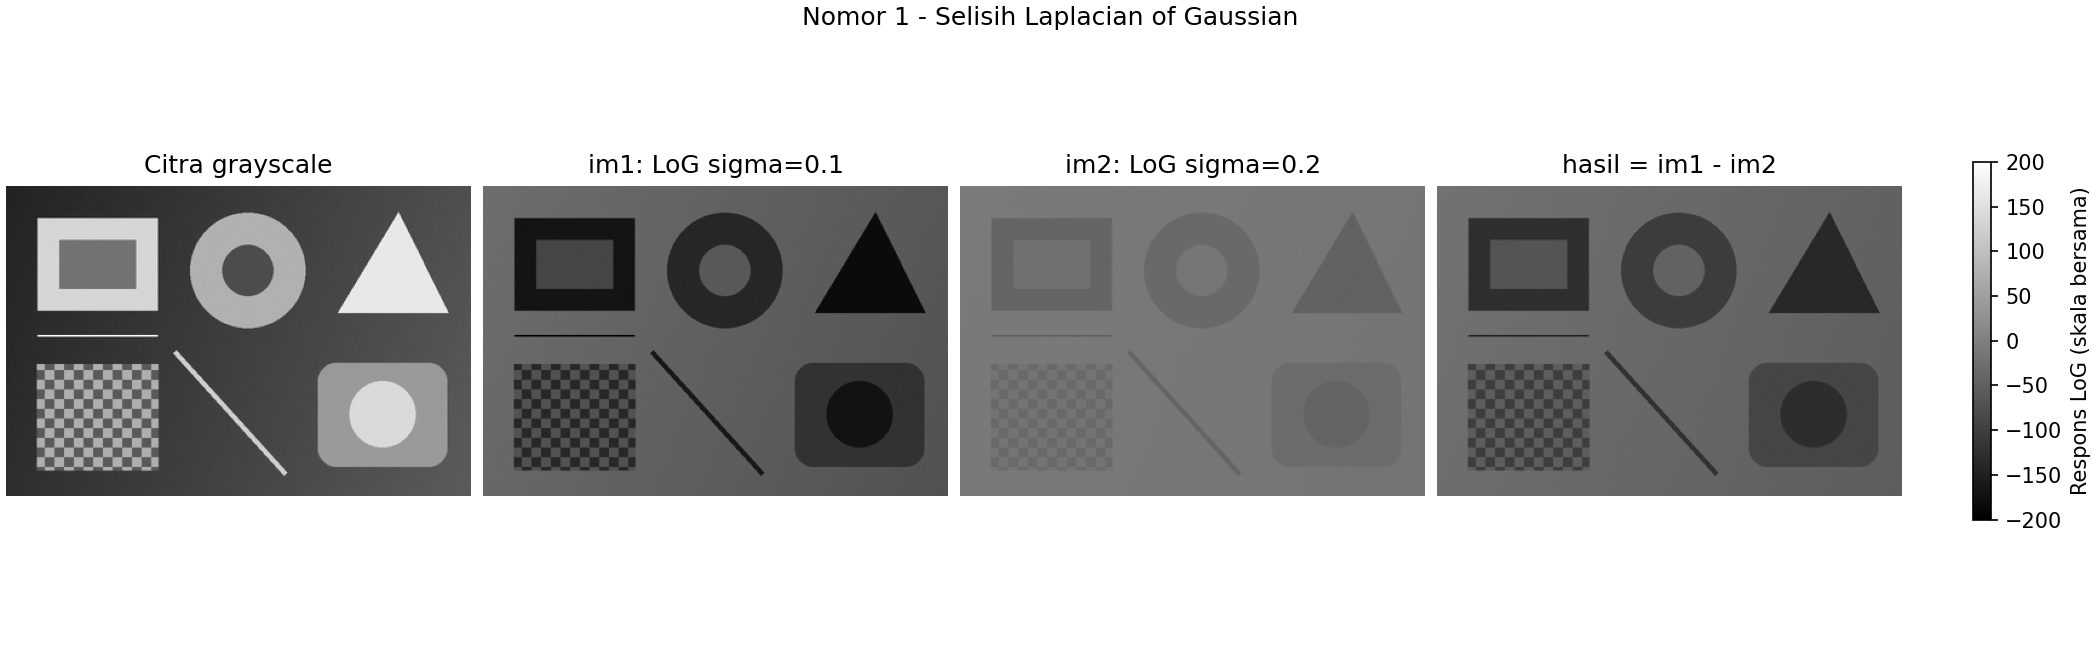
\includegraphics[width=\textwidth]{images/log-perbandingan.png}
\caption{Citra grayscale dan hasil pengolahan nomor 1. Ketiga respons
memakai skala bersama, sedangkan citra grayscale memakai rentang $[0,1]$.}
\label{fig:log-perbandingan}
\end{figure}

\begin{table}[H]
\centering
\caption{Rentang respons asli pada citra contoh, dibulatkan enam desimal.}
\label{tab:log-rentang}
\begin{tabular}{@{}lrr@{}}
\toprule
\textbf{Array} & \textbf{Minimum} & \textbf{Maksimum} \\
\midrule
\kode{im1} & $-200{,}000000$ & $-18{,}039216$ \\
\kode{im2} & $-49{,}994045$ & $-4{,}507871$ \\
\kode{hasil} & $-150{,}006577$ & $-13{,}531345$ \\
\bottomrule
\end{tabular}
\end{table}

Tabel~\ref{tab:log-rentang} berasal dari \kode{metadata.json}, yang juga
mencatat sigma, ukuran citra, metode batas, dan rentang PNG. Pada data
contoh ini $M$ sekitar 200 dan seluruh respons bernilai negatif. Karena
skala tampilan dipakai bersama, perbedaan kecerahan antarpanel pada
Gambar~\ref{fig:log-perbandingan} mencerminkan perbedaan besar respons.

\subsection{Interpretasi sigma kecil dan keterbatasan}

LoG kontinu ideal memberikan respons nol pada citra konstan. Akan tetapi,
sigma $0{,}1$ dan $0{,}2$ jauh lebih kecil daripada jarak antarpiksel.
Pada implementasi SciPy 1.15.3 dengan pemotongan kernel bawaan
\kode{truncate=4}, sigma $0{,}1$ menghasilkan radius kernel nol.
Dalam dua dimensi, respons diskretnya menjadi
$L_{0.1}(I)=-2I/(0{,}1)^2=-200I$, hingga galat pembulatan numerik.
Untuk sigma $0{,}2$, respons pada citra konstan $I=c$ adalah sekitar
$L_{0.2}(c)=-49{,}9906834c$.

Sebagai pemeriksaan, citra konstan $c=0{,}4$ menghasilkan
\kode{im1} sebesar $-80$, \kode{im2} sekitar $-19{,}9962734$, dan
selisih sekitar $-60{,}0037266$. Selisih yang tidak nol ini merupakan
\textbf{bias DC akibat sampling kernel}. Oleh karena itu, hasil bawaan
dapat menyerupai negatif citra dan tidak ditafsirkan semata-mata sebagai
peta tepi. Program tetap menyajikan hasil dengan sigma yang ditentukan
soal, disertai array asli dan penjelasan keterbatasan diskretisasinya.

\clearpage
\subsection{Uji tambahan pada foto nyata}
\label{sec:log-foto-nyata}

Selain citra sintetis, program diuji pada foto grayscale
\kode{skimage.data.camera()} berukuran $512\times512$ piksel.
Foto ini dilisensikan CC0 oleh fotografer Lav Varshney menurut
dokumentasi scikit-image~\cite{skimage-camera}. Salinan foto tanpa perubahan
tersedia pada \kode{soal1/data/foto_kamera_scikit.png}.
Program dan parameter utama dipertahankan: $\sigma_1=0{,}1$,
$\sigma_2=0{,}2$ piksel, mode batas \kode{reflect}, serta
\kode{hasil = im1 - im2}. Kedua filter menerima foto masukan yang sama.

\begin{lstlisting}[style=terminal]
.\.venv\Scripts\python.exe soal1/main.py --input soal1/data/foto_kamera_scikit.png --output-dir soal1/hasil_foto_nyata
\end{lstlisting}

\begin{figure}[H]
\centering
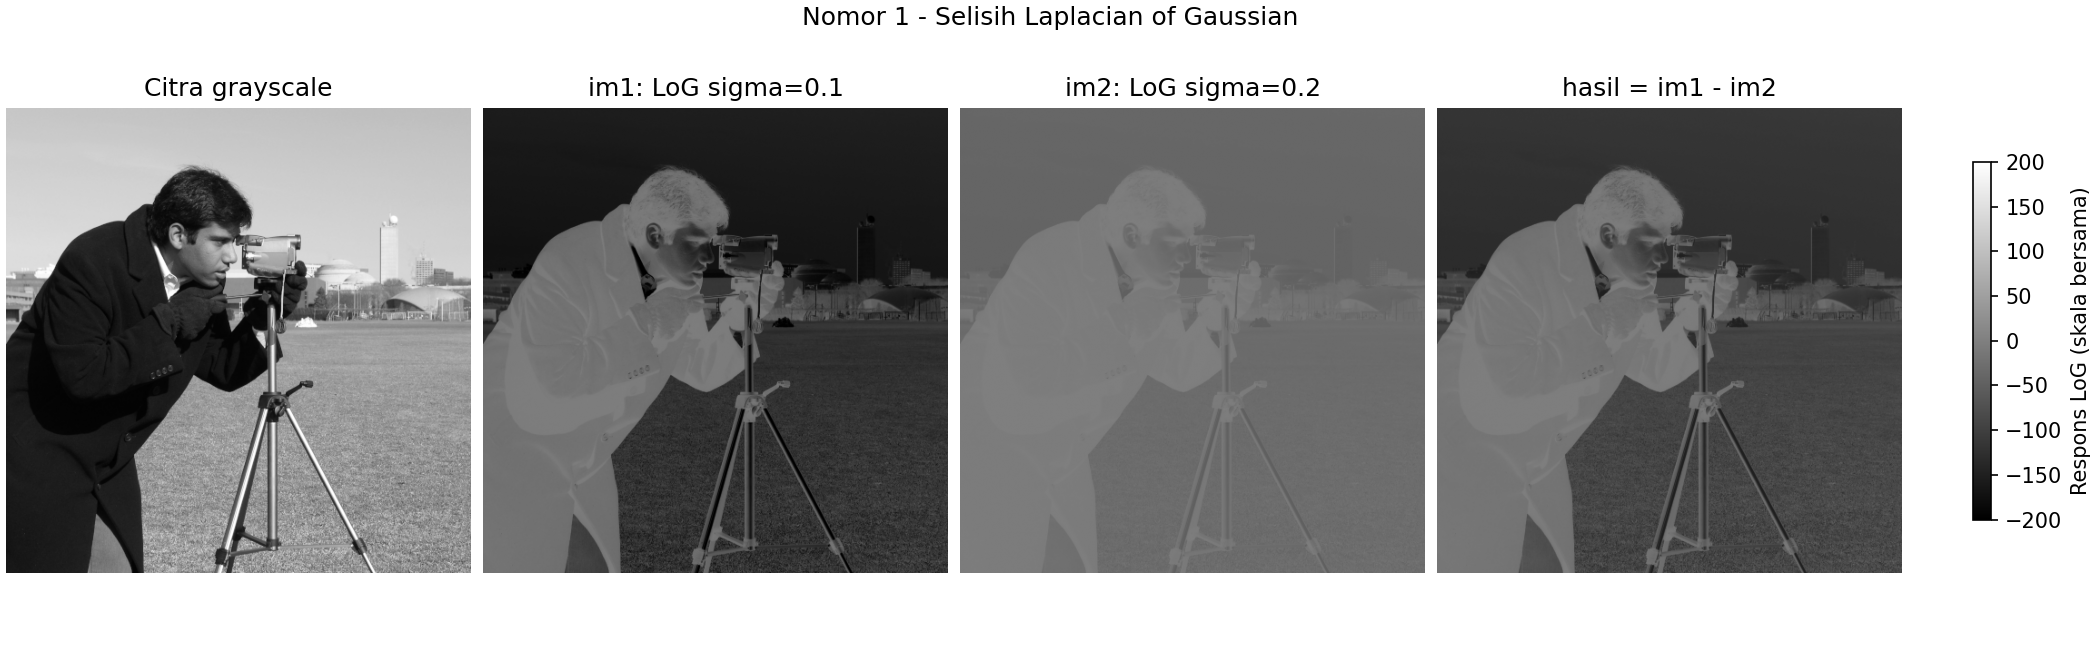
\includegraphics[width=\textwidth]{images/log-foto-nyata.png}
\caption{Dari kiri: foto nyata masukan, respons LoG sigma $0{,}1$,
respons LoG sigma $0{,}2$, dan selisihnya. Ketiga respons menggunakan
skala tampilan bersama.}
\label{fig:log-foto-nyata}
\end{figure}

\begin{table}[H]
\centering
\caption{Rentang respons pada foto nyata, dibulatkan untuk penyajian.}
\begin{tabular}{@{}lrr@{}}
\toprule
\textbf{Array} & \textbf{Minimum} & \textbf{Maksimum}\\
\midrule
\kode{im1} & $-200{,}000000$ & $0{,}000000$\\
\kode{im2} & $-49{,}992070$ & $0{,}000075629$\\
\kode{hasil} & $-150{,}009317$ & $-0{,}000075629$\\
\bottomrule
\end{tabular}
\end{table}

Pemeriksaan array tersimpan menunjukkan bahwa \kode{hasil.npy} sama
persis dengan pengurangan \kode{im1.npy - im2.npy}; ketiganya bertipe
\kode{float64}. Pada foto ini, korelasi selisih terhadap intensitas masukan
sekitar $-0{,}999999999979$. Selisih masih menyerupai negatif foto,
konsisten dengan bias DC akibat sampling kernel pada sigma sangat kecil.
Menggunakan foto nyata tidak menghilangkan keterbatasan tersebut dan
hasil tidak dinyatakan sebagai peta tepi ideal. Data numerik, PNG, dan
metadata tersedia di \kode{soal1/hasil_foto_nyata/}; hasil sintetis
sebelumnya tetap disimpan terpisah.
